% =============================================================================
% Monografia de TCC — Gateway Semântico ROS 2 → SmartData
% Davi Menegaz Junkes — INE/UFSC — Ciência da Computação
% Classe abntex2, padrão de relatório de Projeto II (Cislaghi).
% =============================================================================

\documentclass[
    12pt,
    oneside,
    a4paper,
    chapter=TITLE,
    section=TITLE,
    brazil
]{abntex2}

% ---------- pacotes ----------
\usepackage[T1]{fontenc}
\usepackage[utf8]{inputenc}
\usepackage{lmodern}
\usepackage{helvet}                  % Arial-like sans serif
\renewcommand{\familydefault}{\sfdefault}
\usepackage{indentfirst}
\usepackage{nomencl}
\usepackage{color}
\usepackage{graphicx}
\usepackage{microtype}
\usepackage{lipsum}                  % (não usado em produção; deixe instalado)
\usepackage{booktabs}
\usepackage{array}
\usepackage{tabularx}
\usepackage{multirow}
\usepackage{listings}
\usepackage{xcolor}
\usepackage{amssymb}
\usepackage{amsmath}
\usepackage{siunitx}
\sisetup{output-decimal-marker={,}, group-separator={.}, group-minimum-digits=4}
\usepackage[brazilian,hyperpageref]{backref}
\usepackage[alf]{abntex2cite}        % padrão ABNT autor-data
\usepackage{csquotes}                % \enquote{...}
\usepackage{tikz}
\usetikzlibrary{arrows.meta,positioning,shapes.geometric,fit,calc}

% ---------- formatação visual ----------
% Títulos de capítulo/seção em 14pt (padrão UFSC/INE).
\renewcommand{\ABNTEXchapterfontsize}{\fontsize{14}{16}\selectfont}
\renewcommand{\ABNTEXsectionfontsize}{\fontsize{14}{16}\selectfont}
\renewcommand{\ABNTEXsubsectionfontsize}{\fontsize{12}{14}\selectfont}
\renewcommand{\ABNTEXsubsubsectionfontsize}{\fontsize{12}{14}\selectfont}

% Espaçamento duplo no corpo do texto.
\OnehalfSpacing
\AtBeginDocument{\setlength{\parindent}{1.25cm}}

% Cabeçalho enxuto: sem filete, sem texto, apenas o número da página
% no canto superior (direito em oneside, externo em twoside).
\makeevenhead{abntheadings}{\thepage}{}{}
\makeoddhead{abntheadings}{}{}{\thepage}
\makeheadrule{abntheadings}{\textwidth}{0pt}

% ---------- listings (códigos) ----------
\definecolor{codebg}{rgb}{0.97,0.97,0.97}
\definecolor{codecmt}{rgb}{0.30,0.55,0.30}
\definecolor{codekw}{rgb}{0.10,0.10,0.55}
\lstdefinestyle{codestyle}{
    backgroundcolor=\color{codebg},
    basicstyle=\ttfamily\footnotesize,
    keywordstyle=\color{codekw}\bfseries,
    commentstyle=\color{codecmt}\itshape,
    numbers=left,
    numberstyle=\tiny\color{gray},
    numbersep=8pt,
    breaklines=true,
    showstringspaces=false,
    captionpos=b,
    frame=single,
    framerule=0pt,
    xleftmargin=12pt,
    aboveskip=10pt, belowskip=10pt
}
\lstset{style=codestyle}

% ---------- dados do trabalho ----------
\titulo{Gateway Semântico para Tradução de Mensagens ROS 2
        para o Formato SmartData}
\autor{Davi Menegaz Junkes}
\local{Florianópolis}
\data{2026}
\orientador[Orientador:~]{Prof. Antônio Augusto Fröhlich, Phd.}
\coorientador[Coorientador:~]{Matheus Wagner, Me.}
\instituicao{Universidade Federal de Santa Catarina --- UFSC \par
    Centro Tecnológico --- CTC \par
    Departamento de Informática e Estatística --- INE \par
    Curso de Ciência da Computação}
\tipotrabalho{Trabalho de Conclusão de Curso}
\preambulo{Trabalho de Conclusão de Curso submetido ao Curso de Graduação em
Ciência da Computação do Centro Tecnológico da Universidade Federal de Santa
Catarina como requisito para obtenção do título de Bacharel em Ciência da
Computação.}

% Membros da banca examinadora (preencher antes da defesa).
\newcommand{\membrobancaum}{José Luis Conradi Hoffmann, Phd.}
\newcommand{\membrobancaumfuncao}{Avaliador}
\newcommand{\membrobancauminst}{Universidade Federal de Santa Catarina}

% ---------- hyperref ----------
\makeatletter
\hypersetup{
    pdftitle={\@title},
    pdfauthor={\@author},
    pdfsubject={\imprimirpreambulo},
    pdfkeywords={ROS 2, SmartData, Sistemas Ciber-Físicos,
                 Interoperabilidade Semântica, UDP Multicast},
    colorlinks=true,
    linkcolor=black,
    citecolor=black,
    filecolor=black,
    urlcolor=black,
    bookmarksdepth=4
}
\makeatother

% ===========================================================================
\begin{document}
\selectlanguage{brazil}
\frenchspacing


% ---------- elementos pré-textuais ----------
\pretextual

% ----- capa -----
\begin{capa}
\centering
\fontsize{12}{14}\selectfont
UNIVERSIDADE FEDERAL DE SANTA CATARINA\\
CENTRO TECNOLÓGICO\\
DEPARTAMENTO DE INFORMÁTICA E ESTATÍSTICA\\
CIÊNCIA DA COMPUTAÇÃO\\[4cm]

{\fontsize{12}{14}\selectfont \imprimirautor}\\[4cm]

{\fontsize{14}{16}\selectfont\bfseries \imprimirtitulo}

\vfill
{\fontsize{12}{14}\selectfont \imprimirlocal}\\
{\fontsize{12}{14}\selectfont \imprimirdata}
\end{capa}

% ----- folha de rosto -----
\begin{folhaderosto}
\begin{center}
{\fontsize{12}{14}\selectfont \imprimirautor}\\[6cm]

{\fontsize{14}{16}\selectfont\bfseries \imprimirtitulo}\\[3cm]
\end{center}

\hspace*{0.4\textwidth}%
\begin{minipage}{0.6\textwidth}
\fontsize{12}{14}\selectfont
\SingleSpacing
\imprimirpreambulo

\vspace{1em}
\imprimirorientadorRotulo~\imprimirorientador

\imprimircoorientadorRotulo~\imprimircoorientador
\end{minipage}

\vfill
\begin{center}
{\fontsize{12}{14}\selectfont \imprimirlocal}\\
{\fontsize{12}{14}\selectfont \imprimirdata}
\end{center}
\end{folhaderosto}

% ----- folha de aprovação -----
\begin{folhadeaprovacao}
\centering
{\fontsize{12}{14}\selectfont \imprimirautor}\\[1cm]
{\fontsize{14}{16}\selectfont\bfseries \imprimirtitulo}\\[2cm]

\begin{minipage}{0.85\textwidth}
\fontsize{12}{14}\selectfont
\SingleSpacing
Este Trabalho de Conclusão de Curso foi julgado adequado para obtenção do
Título de Bacharel em Ciência da Computação e aprovado em sua forma final
pelo curso de Graduação em Ciência da Computação.
\end{minipage}\\[1.5cm]

{\fontsize{12}{14}\selectfont Florianópolis, \rule{2cm}{0.4pt} de
\rule{3.5cm}{0.4pt} de \imprimirdata.}\\[2cm]

\begin{center}
\fontsize{12}{14}\selectfont
Banca Examinadora:\\[1.5cm]

\imprimirorientador\\
Orientador\\
Universidade Federal de Santa Catarina\\[1cm]

\imprimircoorientador\\
Coorientador\\
Universidade Federal de Santa Catarina\\[1cm]

\membrobancaum\\
\membrobancaumfuncao\\
\membrobancauminst
\end{center}
\end{folhadeaprovacao}

% ----- resumo -----
\begin{resumo}
A convergência entre robótica móvel e Internet das Coisas é central para a
implementação dos Sistemas Ciber-Físicos. O \textit{Robot Operating System 2}
(ROS 2) consolidou-se como o padrão no desenvolvimento robótico e
adotou o \textit{Data Distribution Service} (DDS) como \textit{middleware}
de comunicação, garantindo entrega eficiente de mensagens. As mensagens
nativas do ROS, porém, transmitem dados brutos de sensores sem o contexto
físico e temporal necessário para sistemas de tomada de decisão autônoma.
O conceito de \textit{SmartData}, proposto por Fröhlich (2018), responde a
essa lacuna ao encapsular cada leitura sensorial em um envelope que carrega,
inseparavelmente do valor, sua unidade no Sistema Internacional, a origem
espaço-temporal do dado e seu prazo de validade. Este trabalho projeta,
implementa e avalia um \textit{Gateway} semântico que opera como nó ROS 2 e
traduz mensagens de sensores robóticos para o formato SmartData. A solução
adota uma estratégia de geração de código em tempo de compilação a partir
de um arquivo declarativo: um descritor YAML enumera os tópicos a converter
e suas regras de decomposição, e um gerador em Python emite os quatro
\textit{headers} C++ que realizam a tradução. O pacote SmartData resultante é
difundido em um barramento UDP
multicast binário de 72~bytes, compatível com transdutores SmartData
externos. A validação empírica em ambiente conteinerizado mediu uma latência
de \textit{marshaling} de \SI{0.8}{\micro\second} no 95º percentil para uma
mensagem de varredura LiDAR de 100 feixes, valor três ordens de grandeza
abaixo do piso de latência do ROS 2 para cargas pequenas reportado na
literatura, entre \SI{1}{\milli\second} e \SI{3}{\milli\second}. Os resultados
sustentam a viabilidade de integrar robôs ROS 2 a ecossistemas SmartData
sem comprometer o desempenho do laço de controle.

\vspace{1cm}
\noindent\textbf{Palavras-chave:}
ROS 2; SmartData; Sistemas Ciber-Físicos; Interoperabilidade Semântica;
Tradução Semântica; UDP Multicast.
\end{resumo}

% ----- sumário e listas -----
\pdfbookmark[0]{\contentsname}{toc}
\tableofcontents*
\cleardoublepage

% ===========================================================================
\textual

% ===========================================================================
\chapter{Introdução}
\label{cap:introducao}

A evolução dos Sistemas Ciber-Físicos (\textit{Cyber-Physical Systems},
CPS) e a consolidação da Internet das Coisas transformaram a forma como
máquinas interagem com o mundo físico. Como argumenta \citeonline{lee2008cps},
a essência dos CPS reside na orquestração integrada de computação,
comunicação e controle, onde a dinâmica dos processos físicos exige o mesmo
rigor formal que as computações lógicas. Nesse cenário, a robótica móvel
deixou de operar como sistema isolado e tornou-se um componente ativo em
ambientes inteligentes, integrada a infraestruturas de instrumentação,
controle e analítica que extrapolam os limites do robô.

No domínio do desenvolvimento robótico, o \textit{Robot Operating System}
(ROS) estabeleceu-se como o padrão de fato para a construção de sistemas
complexos. O ROS 2 introduziu uma mudança arquitetural significativa ao
substituir seu transporte próprio pelo \textit{Data Distribution Service}
(DDS), um padrão da OMG voltado a sistemas distribuídos de tempo real
\cite{maruyama2016ros2,macenski2022ros2}. Paralelamente, no contexto de
IoT industrial e cidades inteligentes, o conceito de \textit{SmartData},
proposto por \citeonline{frohlich2018smartdata}, oferece uma abordagem
orientada a dados que enriquece a informação bruta com metadados de
semântica, localização e validade temporal, tornando cada leitura sensorial
um objeto autocontido.

Apesar de coexistirem no mesmo nicho de aplicações ciber-físicas, os dois
modelos de dados operam em níveis distintos de abstração. As mensagens
nativas do ROS são projetadas para a eficiência do laço de controle
e expõem campos numéricos ou estruturas pouco anotadas, das quais o
significado semântico, como, unidade física, validade temporal e referencial
espaço-temporal, é convenção do projeto, não dependente da
mensagem. O SmartData, por sua vez, encapsula essas informações no próprio
envelope, mas é difundido em um barramento próprio incompatível com o
ferramental ROS. \citeonline{serrano2015stack} caracterizam esse isolamento como um dos
problemas centrais à interoperabilidade na Internet das Coisas, padrão que
se reproduz na fronteira entre robótica e instrumentação ciber-física e
motiva a tradução proposta neste trabalho.

\section{Problema de Pesquisa}
\label{sec:problema}

A motivação deste trabalho está na ausência de um mecanismo direto e
eficiente de tradução entre as mensagens operacionais do ROS 2 e o formato
semanticamente enriquecido do SmartData. \textit{Gateways} de aplicação
genéricos existem, mas tipicamente introduzem latência incompatível com
laços de controle robóticos ou perdem metadados durante a serialização.
Formula-se, portanto, a seguinte questão de pesquisa: como viabilizar a
interoperabilidade semântica entre sistemas robóticos baseados em ROS 2 e
plataformas de CPS orientadas a SmartData, mantendo os requisitos de tempo
real e baixo \textit{overhead} de processamento?

\section{Hipótese}
\label{sec:hipotese}

Este trabalho conjectura que é possível desenvolver um componente operando
nativamente no ecossistema ROS 2 capaz de interceptar, enriquecer e
retransmitir mensagens de sensores no formato SmartData, com uma latência
de \textit{marshaling} pequena o suficiente para não afetar o funcionamento
dos demais subsistemas. Assume-se que, ao realizar a tradução dentro do
próprio nó ROS, aproveitando as proprias informações do ecossistema
para preencher os metadados  referentes de uma mensagem 
SmartData, elimina-se a necessidade de \textit{brokers} externos
complexos, preservando a integridade semântica dos dados.

\section{Justificativa}
\label{sec:justificativa}

A relevância desta pesquisa decorre da transição da arquitetura de sistemas
robóticos para ecossistemas conectados e centrados em dados. A maturidade
alcançada pelo ROS 2 \cite{macenski2022ros2} resolveu problemas críticos
de descoberta, escalabilidade e qualidade de serviço no transporte, mas
não endereçou nativamente a compreensão semântica da informação: o
\textit{middleware} garante a entrega da mensagem, não que o receptor
interprete inequivocamente a unidade física, o referencial de coordenadas
ou a validade temporal do dado sem configuração prévia manual.

A lacuna semântica representa risco para a segurança e a confiabilidade de
sistemas autônomos heterogêneos. \citeonline{prestes2013ontology} apontam
que a falta de uma ontologia padronizada e acoplada aos dados em tempo de
execução é causa frequente de falhas na composição de robôs de fabricantes
ou módulos distintos. O SmartData mitiga esse risco ao acoplar
inseparavelmente o valor numérico aos seus metadados de semântica, espaço e
tempo \cite{frohlich2018smartdata}. Do ponto de vista de desempenho,
executar a tradução dentro do próprio processo ROS, e não em um processo
externo encadeado por mais uma travessia de serialização, preserva a
viabilidade do caminho para laços de controle em tempo real
\cite{kronauer2021latency}.

\section{Objetivos}
\label{sec:objetivos}

\subsection{Objetivo Geral}
Projetar, implementar e validar experimentalmente um \textit{Gateway}
semântico para ROS 2 capaz de interceptar mensagens de sensores padrão e
retransmiti-las em tempo real no formato SmartData, preservando a
integridade semântica, espacial e temporal dos dados originais.

\subsection{Objetivos Específicos}
\begin{enumerate}
    \item Definir um modelo formal de correspondência entre mensagens de
    sensores ROS e a estrutura tipada do SmartData, expressível por meio
    de um arquivo declarativo.
    \item Implementar o \textit{Gateway} como nó nativo do ROS 2,
    aproveitando a árvore de transformações e o relógio do próprio
    ecossistema para enriquecer cada amostra com sua origem espaço-temporal.
    \item Difundir o SmartData produzido em um barramento binário UDP
    multicast compatível com transdutores SmartData nativos, oferecendo
    como caminho secundário um espelhamento em tópico ROS para
    instrumentação e depuração no próprio ecossistema.
    \item Caracterizar empiricamente a latência de \textit{marshaling} e a
    vazão sustentada do tradutor, a partir exclusivamente do
    barramento SmartData.
\end{enumerate}

\subsection{Escopo e Limites}
A pesquisa delimita-se à camada de \textit{software} de aplicação sobre
ROS 2 Humble em Linux, tratando o DDS subjacente apenas como o transporte
padrão do ROS, sem propor modificações ao \textit{middleware}. A validação
restringe-se a cenários simulados (gerador sintético e Gazebo) para garantir a
reprodutibilidade. Mecanismos criptográficos previstos pelo SmartData
estão fora do escopo deste trabalho, que se concentra na estrutura de
dados e na caracterização de desempenho.

% ===========================================================================
\chapter{Fundamentação Teórica}
\label{cap:fundamentacao}

Este capítulo apresenta os três pilares conceituais sobre os quais o
\textit{Gateway} foi construído: Sistemas Ciber-Físicos como contexto da
demanda por dados semanticamente ricos, o ROS 2 como plataforma robótica
baseada em DDS, e o conceito de SmartData como construção de envelope para
dados de sensores. Cada seção descreve as definições, propriedades e
limitações que motivaram decisões de projeto adotadas nos capítulos
posteriores.

\section{Sistemas Ciber-Físicos}
\label{sec:cps}

Sistemas Ciber-Físicos são, na definição de \citeonline{lee2008cps},
integrações de computação e processos físicos nas quais computadores
embarcados e redes monitoram e controlam o mundo físico, comumente em
laços de realimentação. O autor argumenta que a passagem do tempo, no mundo
físico, é inevitável e a concorrência é intrínseca; ambas as propriedades,
no entanto, não são tratadas pelas abstrações usuais,
herdadas da computação de propósito geral. As consequências práticas
incluem a dificuldade de raciocinar formalmente sobre latência, determinismo
e ordenação em sistemas que mediam controle físico.

A demanda por confiabilidade em CPS é qualitativamente distinta da
encontrada em \textit{software} convencional. Em uma aplicação de
processamento de texto, uma falha pode produzir desconforto, já em um sistema
de controle automotivo, ela pode produzir danos físicos. Lee enfatiza que
as decisões de projeto em CPS devem incorporar explicitamente o tempo e a
concorrência como cidadãos de primeira classe, e não como propriedades
emergentes da implementação. Esse argumento da base à adoção de mecanismos
como o \textit{Data Distribution Service} pelo ROS 2 e ao enriquecimento
temporal dos pacotes SmartData no presente trabalho.

\section{Robot Operating System 2}
\label{sec:ros2}

O ROS é um conjunto de bibliotecas e ferramentas para o desenvolvimento de
sistemas robóticos; o ROS 2 é seu sucessor, redesenhado para abordar
limitações herdadas da primeira versão em segurança, tempo real e
operação em redes não ideais \cite{macenski2022ros2}. A diferença
arquitetural mais relevante para este trabalho é a substituição do
transporte original do ROS 1 pelo DDS, um padrão da \textit{Object
Management Group} para comunicação dirigida a dados, baseado no modelo
publish/subscribe com descoberta distribuída e configurações de qualidade
de serviço (QoS) \cite{maruyama2016ros2}.

\subsection{Modelo de Comunicação}
No modelo de comunicação do ROS 2, processos (\textit{nodes}) publicam e
assinam tópicos identificados por nome e tipo de mensagem. Cada tipo de
mensagem é definido em uma linguagem de descrição de interface, a
\textit{Interface Definition Language} (IDL) usada pelo DDS, e
compilado a estruturas de dados nativas em C++ e Python. O publicador
serializa uma instância da mensagem segundo o IDL e a entrega à camada
DDS, que a roteia para todos os assinantes interessados de acordo com a
política de QoS associada ao tópico.

A qualidade de serviço é configurável por tópico e abrange, entre outros,
profundidade do histórico, confiabilidade (\textit{reliable} ou
\textit{best-effort}), durabilidade e prazos. O ROS 2 oferece perfis
nomeados como \texttt{SensorDataQoS}, otimizado para dados sensoriais de
alta frequência, e \texttt{SystemDefaultsQoS}, que herda a configuração
padrão do \textit{middleware}.

\subsection{Implementação por Camadas}
A pilha do ROS 2 segue uma estratificação clara
\cite{macenski2022ros2,maruyama2016ros2}. Bibliotecas cliente como
\texttt{rclcpp} expõem o modelo de \textit{publish}/\textit{subscribe} ao
programador e delegam a comunicação a um \textit{middleware interface
module} (\texttt{rmw}), que por sua vez encapsula uma implementação
concreta de DDS, como Fast~DDS, Cyclone~DDS ou Connext. A separação
entre \texttt{rmw} e a implementação de DDS permite que o mesmo código de
aplicação rode sobre fornecedores distintos.

\subsection{Caracterização de Desempenho}
A latência de comunicação do ROS 2 foi caracterizada em diversos estudos.
\citeonline{maruyama2016ros2} mostraram que a sobrecarga da pilha do ROS 2
sobre o DDS bruto varia significativamente conforme o cenário, com valores
da ordem de centenas de microssegundos para mensagens pequenas em
processos distintos. \citeonline{kronauer2021latency} estenderam essa
análise para sistemas com múltiplos nós e mostraram que o ROS 2 pode
introduzir até 50\% de \textit{overhead} sobre o DDS bruto para mensagens
pequenas, com valores típicos no 95º percentil entre uma e três
milissegundos para cargas de \SI{128}{\byte} a \SI{500}{\kilo\byte} em
configurações representativas. Esses dados são a referência mais
diretamente comparável ao \textit{overhead} adicional que um tradutor
para SmartData deve evitar reintroduzir.

\subsection{Árvore de Transformações}
O subsistema \texttt{tf2} do ROS mantém uma árvore de transformações
geométricas entre quadros de referência, indexada no tempo. Cada par de
quadros é vinculado por uma transformação contínua, e consultas sobre essa
árvore retornam, para um instante específico, a transformação resultante
da composição ao longo de um caminho da árvore. Essa estrutura é a fonte
canônica para preencher os campos de origem espacial do SmartData a partir
do \texttt{frame\_id} declarado no cabeçalho das mensagens de sensor.

\section{O Conceito de SmartData}
\label{sec:smartdata}

O SmartData foi proposto por \citeonline{frohlich2018smartdata} como a
abstração primária usada por aplicações para
interagir com o mundo físico em uma rede de sensores e atuadores. Trata-se
de um dado enriquecido com metadados suficientes para ser autocontido
quanto à semântica, à localização espacial, ao instante de produção e à
confiabilidade. Conceitualmente, ler uma instância de SmartData implica
amostrar o transdutor associado, e escrever em uma instância define um novo
\textit{setpoint} para um atuador.

\subsection{Estrutura do Envelope}
Cada envelope SmartData carrega, além do valor numérico, uma unidade
codificada como inteiro de 32 bits que descreve a dimensão SI da grandeza
sensoriada, as coordenadas \((x, y, z)\) da origem espacial, um
\textit{timestamp} de alta resolução, um prazo de validade
(\textit{expiry}) relativo ao instante de produção e um código de
autenticação. A unidade é codificada com um bit de tipo (físico/digital),
dois bits para o tipo numérico, dois bits para um modificador (direto,
inverso, logarítmico) e nove campos de três bits para os expoentes das
sete dimensões fundamentais do SI mais radiano e esterradiano, conforme
ilustrado na Figura~1 do trabalho original.

Essa codificação produz, por exemplo, a constante \texttt{METER} com
expoente \(+1\) na dimensão de comprimento e zero nas demais;
\texttt{METER\_PER\_SEC\_SQ} com expoentes \(+1\) em comprimento e \(-2\)
em tempo, descrevendo aceleração; e \texttt{VOLT} como composto das
dimensões de massa, comprimento, tempo e corrente segundo a definição
formal. Portanto, a semântica é intrínseca ao identificador de unidade,
sem necessidade de tabelas de tradução externas.

\subsection{Origem Espaço-Temporal e Validade}
O \textit{timestamp} de origem é expresso em microssegundos contados a
partir de uma época absoluta, por padrão, a época UNIX. A validade
relativa permite que o consumidor avalie, a qualquer instante, se o dado
ainda é semanticamente utilizável: um valor lido após o vencimento foi
produzido em um ponto do passado em que as condições físicas observadas
podem já não corresponder ao estado atual do sistema. Em
\citeonline{frohlich2019datacentric}, a validade é discutida como um
substituto operacional para os prazos de tarefas em escalonadores de tempo
real, deslocando o raciocínio temporal da execução para os dados.

\subsection{Endereçamento e Discriminação por Faixas de Dispositivo}
O envelope SmartData inclui um identificador \texttt{origin\_device} que
disambigua múltiplas fontes da mesma grandeza física. Esse campo será
empregado, no projeto descrito no Capítulo~\ref{cap:design}, como
mecanismo de roteamento: cada sensor traduzido recebe uma faixa
disjunta de dispositivos, e o consumidor escolhe o reconstrutor correto
combinando a unidade com a faixa do dispositivo.

% ===========================================================================
\chapter{Trabalhos Relacionados}
\label{cap:relacionados}

A literatura adjacente a este trabalho organiza-se em três frentes:
caracterizações de desempenho do ROS 2 e do DDS, propostas de
interoperabilidade semântica para a Internet das Coisas e implementações
do conceito de SmartData em pilhas de comunicação industriais. Esta
seção discute cada frente e posiciona a contribuição da presente
monografia em relação a elas.

\section{Desempenho de Middleware Robótico}
\label{sec:rel-perf}

\citeonline{maruyama2016ros2} produziram a primeira caracterização
sistemática do desempenho do ROS 2 sobre DDS. Os autores descrevem a
arquitetura em camadas, comparam fornecedores e medem latência e vazão
sob configurações variáveis de QoS, tamanho de mensagem e número de
processos. Sua contribuição central é demonstrar que o desempenho do
ROS 2 depende fortemente do par \textit{rmw}/DDS escolhido e da
configuração de QoS, e que ganhos significativos podem ser obtidos pela
seleção criteriosa desses parâmetros para o cenário de aplicação.

\citeonline{kronauer2021latency} estenderam a análise para sistemas com
múltiplos nós e quantificaram a sobrecarga adicionada pela pilha do ROS 2
em relação ao DDS bruto. Encontraram que, para mensagens pequenas
(da ordem de \SI{128}{\byte}), o ROS 2 chega a duplicar a latência
percebida em comparação com chamadas diretas ao DDS, principalmente em
razão das filas internas e da indireção das interfaces \texttt{rmw}.
Para mensagens grandes, a fração relativa do \textit{overhead} encolhe e
o gargalo migra para o próprio DDS.

A relevância desses resultados para o presente trabalho é direta. Um
tradutor que se interponha entre a mensagem ROS original e o consumidor
SmartData não pode replicar dentro do seu processo o mesmo
\textit{overhead} que a pilha já paga. As decisões de projeto descritas
no Capítulo~\ref{cap:design}, subscrição tipada na própria pilha
\texttt{rclcpp}, ausência de introspecção em tempo de execução e
barramento UDP binário sem intermediação por DDS, são respostas
diretas a essa preocupação.

\section{Interoperabilidade Semântica em IoT}
\label{sec:rel-semantic}

\citeonline{serrano2015stack} discutem a fragmentação do ecossistema de
Internet das Coisas em silos verticais que não interoperam e propõem uma
pilha de orquestração baseada em \textit{middleware} semântico, o
OpenIoT-VDK. A estratégia dos autores é: introduz camadas de
anotação, filtragem e agregação em um \textit{broker} central que media
o acesso a sensores virtuais e físicos. A abordagem é eficaz em cenários
de coleta de dados em escala urbana, mas é incompatível com a latência
exigida por laços de controle robótico, pois cada amostra atravessa
processos adicionais antes de chegar ao consumidor.

O presente trabalho herda a motivação, interoperabilidade semântica
entre subsistemas heterogêneos, mas adota uma abordagem
arquitetonicamente oposta: a tradução ocorre dentro do mesmo processo
que assina o tópico ROS, sem \textit{brokers} externos, e o consumidor
SmartData recebe o envelope diretamente do barramento, sem intermediação
adicional. A solução é mais restrita em escopo (não trata de agregação
nem de consulta histórica), mas adequada ao domínio robótico.

\section{Implementações de SmartData}
\label{sec:rel-smartdata}

O conceito de SmartData foi originalmente proposto e implementado por
\citeonline{frohlich2018smartdata} no contexto do \textit{Embedded
Parallel Operating System} (EPOS) e do \textit{Trustful Space-Time
Protocol} (TSTP), uma pilha de rede própria para sensores embarcados. A
implementação original endereçava nós embarcados de baixíssimo consumo
energético, com o EPOS abstraindo transdutores como objetos C++ e o TSTP
provendo entrega segura e sincronizada. Essa origem moldou a estrutura
do envelope: a presença do campo de validade, a codificação compacta da
unidade e o tamanho fixo do pacote refletem decisões orientadas a redes
de sensores com restrições severas de banda.

Em \citeonline{frohlich2019datacentric}, o conceito é estendido para o
projeto de CPS completos, com discussão sobre escalonamento orientado a
dados, no qual tarefas são executadas para produzir os SmartData
demandados antes que expirem. Essas implementações compartilham a
estratégia de produzir SmartData diretamente em transdutores embarcados,
abaixo de qualquer pilha de aplicação.

A contribuição original deste trabalho complementa essas implementações
ao oferecer a ponte que faltava no sentido oposto: a entrada do
ecossistema robótico. Enquanto as implementações anteriores produziam
SmartData em transdutores embarcados e os consumiam em aplicações
industriais, este trabalho posiciona o gateway no ponto em que mensagens
ROS já existentes precisam ser elevadas semanticamente para alcançar
consumidores SmartData, sem demandar reescrita dos sensores ou do
ferramental robótico.

% ===========================================================================
\chapter{Design do Sistema}
\label{cap:design}

Este capítulo descreve a arquitetura do \textit{Gateway} semântico e as
decisões de projeto que conduziram à sua forma final. A apresentação parte
de uma visão geral do fluxo de dados, detalha a linguagem declarativa que
descreve cada sensor, discute a estratégia de geração de código e justifica a
existência de dois transportes complementares.

\section{Visão Geral}
\label{sec:visao}

O Gateway é composto por dois executáveis ROS 2, um por sentido da
tradução, e por uma biblioteca de transporte independente do
\textit{middleware} do ROS, baseada em sockets UDP multicast. O primeiro
executável, \texttt{gateway\_node}, realiza a tradução direta:
assina os tópicos de sensores declarados no descritor, decompõe cada
mensagem recebida em uma sequência de envelopes SmartData e os emite por
dois canais paralelos. O segundo, \texttt{sd\_to\_ros\_node}, realiza a
tradução inversa: escuta o barramento binário, agrega os envelopes que
compartilham origem temporal e republica a mensagem ROS correspondente
em um tópico tipado. 

A figura conceitual do fluxo é a seguinte: uma mensagem ROS chega à
\texttt{Subscription} tipada criada pelo gateway; o \textit{callback}
correspondente consulta a árvore \texttt{tf2} para resolver a origem
espacial associada ao \texttt{frame\_id} da mensagem e produz um vetor
de SmartData. Cada SmartData é então difundido em um grupo UDP multicast
de 72~bytes e, opcionalmente, espelhado em um tópico ROS
\(\texttt{/smartdata/<sensor>}\) do tipo
\texttt{semantic\_gateway/msg/SmartData}. A
Figura~\ref{fig:fluxo-gateway} resume o caminho percorrido por uma
mensagem.

\begin{figure}[htb]
\centering
\caption{Fluxo de tradução no \texttt{gateway\_node}}
\label{fig:fluxo-gateway}
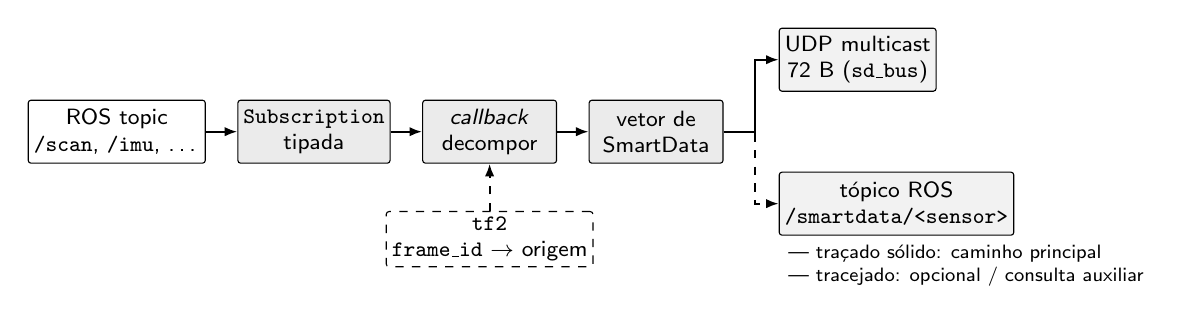
\begin{tikzpicture}[
  font=\footnotesize\sffamily,
  node distance=4mm and 4mm,
  every node/.style={align=center},
  box/.style={draw, rounded corners=1pt, minimum height=8mm,
              minimum width=17mm, inner sep=2pt, fill=black!3},
  proc/.style={box, fill=black!8},
  sink/.style={box, fill=black!5},
  src/.style={box, fill=white},
  aux/.style={draw, dashed, rounded corners=1pt, fill=white,
              minimum height=7mm, inner sep=2pt},
  arr/.style={-{Latex[length=1.6mm]}, thick},
  dashedarr/.style={-{Latex[length=1.6mm]}, thick, dashed},
]

\node[src] (topic) {ROS topic\\ \texttt{/scan}, \texttt{/imu}, \dots};
\node[proc, right=of topic] (sub) {\texttt{Subscription}\\ tipada};
\node[proc, right=of sub] (cb) {\textit{callback}\\ decompor};
\node[aux, below=6mm of cb] (tf) {\texttt{tf2}\\ \texttt{frame\_id} $\to$ origem};
\node[proc, right=of cb] (vec) {vetor de\\ SmartData};

\node[sink, above right=1mm and 7mm of vec] (udp)
      {UDP multicast\\ 72~B (\texttt{sd\_bus})};
\node[sink, below right=1mm and 7mm of vec] (mirror)
      {tópico ROS\\ \texttt{/smartdata/<sensor>}};

\draw[arr] (topic) -- (sub);
\draw[arr] (sub) -- (cb);
\draw[arr] (cb) -- (vec);
\draw[dashedarr] (tf) -- (cb);
\draw[arr] (vec.east) -- ++(4mm,0) |- (udp.west);
\draw[dashedarr] (vec.east) -- ++(4mm,0) |- (mirror.west);

\node[anchor=north west, font=\scriptsize\sffamily, align=left]
      at ($(mirror.south west)+(0, 0)$)
      {\textemdash\ traçado sólido: caminho principal\\
       \textemdash\ tracejado: opcional / consulta auxiliar};

\end{tikzpicture}

\legend{Fonte: elaborada pelo autor.}
\end{figure}

\section{Linguagem Declarativa de Sensores}
\label{sec:dsl}

A configuração do \textit{Gateway} é especificada em um arquivo YAML que
declara, para cada sensor a ser traduzido, o tópico ROS de entrada, o tipo
de mensagem, o padrão de decomposição e parâmetros específicos da
decomposição. Três padrões cobrem os tipos relevantes da biblioteca
\texttt{sensor\_msgs}:

\begin{description}
\item[Escalar] Uma mensagem ROS produz exatamente um SmartData. O campo
\texttt{value\_field} aponta para o atributo numérico a ser extraído, e
um \texttt{value\_transform} linear opcional permite ajustar a unidade
(por exemplo, conversão de graus Celsius para Kelvin pela aplicação de
\(a \cdot v + b\)). A transformação inversa é gerada automaticamente para
o caminho de reconstrução.

\item[Vetor] Uma mensagem ROS produz \(N\) SmartData, um por elemento de
um campo vetorial. O caso prototípico é o \texttt{LaserScan}, cuja
distância de cada feixe vira um SmartData independente endereçado por um
deslocamento de dispositivo. Filtros opcionais (\texttt{finite},
\texttt{finite\_within}) descartam feixes inválidos ou fora da faixa
declarada do sensor.

\item[Composto] Uma mensagem ROS é decomposta em grupos de campos, cada
um com sua própria unidade. O caso prototípico é o \texttt{Imu}, cujos
três componentes de aceleração linear formam um grupo na unidade
\si{\meter\per\square\second} e os três componentes de velocidade
angular formam outro grupo em \si{\radian\per\second}.
\end{description}

Cada sensor declara também um prazo de validade (\texttt{expiry\_ms}),
que é aposto a todos os SmartData produzidos por suas mensagens. A
estampa de tempo do envelope é derivada do campo de cabeçalho ROS
indicado por \texttt{stamp\_field}, e a origem espacial vem da consulta
\texttt{tf2} ao quadro indicado por \texttt{frame\_field}.

\section{Geração de Código em Tempo de Compilação}
\label{sec:codegen}

O problema central desta camada é como associar, em C++, os campos de
uma mensagem ROS 2 aos SmartData produzidos, sabendo que o conjunto de
tipos a traduzir só é fixado quando o descritor YAML é lido. Duas
estratégias respondem a esse problema, com perfis de custo bastante
distintos.

A primeira alternativa é a introspecção de tipos em tempo de
execução, apoiada pelo pacote
\texttt{rosidl\_typesupport\_introspection\_cpp}. Nela, o
\texttt{gateway\_node} carrega o descritor no \textit{startup}, resolve
dinamicamente o tipo de cada mensagem e navega os campos por nome a
cada callback. A vantagem é a flexibilidade: adicionar um sensor não
exige recompilação, e o binário é único para qualquer configuração.
Os custos, porém, são estruturais. A busca por nome ocorre por campo e
por mensagem, o que agrega latência proporcional ao número de campos
extraídos, incompatível com o critério adotado de manter o
\textit{marshaling} abaixo de \SI{100}{\micro\second}, uma ordem de
grandeza abaixo do piso de latência do ROS 2 reportado por
\citeonline{kronauer2021latency}. Além disso, a validação da
configuração é adiada: uma referência a um campo inexistente no YAML
não é detectada na compilação nem na inicialização, mas apenas na
primeira mensagem em que aquele caminho é exercido, o que favorece
falhas silenciosas em produção.

A segunda alternativa é a geração de código em tempo de
compilação. Um gerador em Python lê o descritor YAML e emite
\textit{headers} C++ nos quais cada acesso a campo aparece de forma
literal (por exemplo, \texttt{msg.linear\_acceleration.x}) e cada
\texttt{Subscription} já surge instanciada com seu tipo estático. O
compilador, portanto, pode inspecionar cada rota de tradução, e o
custo por mensagem colapsa em uma sequência de acessos diretos, sem
lookups por nome. Em contrapartida, o descritor participa do processo
de \textit{build}: alterar o YAML exige regenerar os \textit{headers} e
recompilar o \texttt{gateway\_node}. Esse acoplamento entre configuração
e compilação, contudo, é benéfico no contexto deste trabalho, pois
converte erros de descritor em erros do compilador, detectados antes
de o sistema ser posto em operação.

Adotou-se a segunda alternativa. A introspecção seria a escolha natural
se o conjunto de sensores mudasse com frequência em campo, sem janela de
recompilação, porem, nesse gateway, o descritor é parte da configuração
do robô, alterado com pouca frequência e sempre antes do
\textit{deploy}, de modo que o custo de recompilação é raro e o ganho
em latência e em detecção precoce de erros é permanente. O gerador
emite quatro \textit{headers} C++, cada um responsável por uma fatia
bem delimitada do tradutor:

\begin{description}
\item[\texttt{parsed\_decompose.hpp}] Contém uma função
\texttt{decompose\_<topic>} por sensor, especializada no tipo da
mensagem ROS correspondente. O acesso aos campos é direto (por exemplo,
\texttt{msg.linear\_acceleration.x}), sem nenhuma busca por nome em
tempo de execução.

\item[\texttt{parsed\_dispatch.hpp}] Contém a função \texttt{register\_all},
chamada uma vez na inicialização do \texttt{gateway\_node}, que cria as
\texttt{rclcpp::Subscription<T>} tipadas para cada sensor e conecta o
\textit{callback} ao \texttt{decompose\_<topic>} correspondente.

\item[\texttt{parsed\_recompose.hpp}] Contém os estados acumuladores e as
funções \texttt{feed\_<topic>} usadas pelo caminho inverso. Cada estado
é estritamente tipado pela mensagem alvo da reconstrução, e a inversa
do \texttt{value\_transform} declarado é embutida durante a geração.

\item[\texttt{parsed\_sd\_dispatch.hpp}] Contém a estrutura \texttt{Consumers}
e a função \texttt{dispatch\_sd}, que recebe um SmartData arbitrário do
barramento e o entrega ao \texttt{feed\_<topic>} correto.
\end{description}

A geração ocorre via \texttt{add\_custom\_command} do CMake, sendo
disparada automaticamente quando o YAML ou o gerador são modificados.
O resultado é que toda a tradução é resolvida estaticamente: a única dependência de
configuração é o arquivo de cabeçalho gerado, embutido no compilado.

\section{Discriminação por Faixas de Dispositivo}
\label{sec:dev-base}

O barramento UDP multicast transporta SmartData de todos os sensores em
um único grupo, portanto o consumidor precisa identificar a qual
mensagem ROS cada envelope pertence. A solução adotada é alocar uma
faixa disjunta do espaço de \texttt{origin\_device} a cada sensor
declarado, sequencialmente, com tamanho fixo de \(2^{16}\) endereços por
sensor. O sensor de índice \(i\) recebe a faixa
\([i \cdot 2^{16},\,(i+1) \cdot 2^{16})\), e a função
\texttt{dispatch\_sd} roteia um envelope para o consumidor cuja faixa
contém o \texttt{origin\_device} recebido, conjugada à conferência da
unidade esperada.

Essa escolha tem duas propriedades favoráveis: primeiro, mantém o
barramento livre de cabeçalho de identificação adicional, o roteamento é
inferido a partir de campos que já existiriam no envelope SmartData,
segundo, suporta sensores vetoriais com até \(2^{16}\)
elementos, suficiente para LiDARs comerciais de alta resolução.

\section{Transportes do SmartData}
\label{sec:transport}

O \textit{Gateway} emite cada envelope SmartData por dois canais
paralelos cuja coexistência é uma decisão arquitetural deliberada.

\subsection{Barramento UDP Multicast}
O caminho primário é um datagrama UDP multicast de 72 \textit{bytes}
\textit{little-endian} difundido no grupo \texttt{224.1.1.1:5000}. Esse
\textit{layout} corresponde à serialização binária da estrutura
\texttt{SDWire}: cinco campos de origem (\(x, y, z, \texttt{device},
t\)) ocupam 36 \textit{bytes}, a unidade ocupa 4, o valor ocupa 8, a
validade ocupa 8 e a assinatura ocupa 16. A escolha de multicast é 
justificada: descobre dinamicamente consumidores sem
configuração explícita e reflete a semântica de \enquote{interesse em
uma região} do conceito original de SmartData, em que múltiplos nós
podem subscrever o mesmo grupo de unidade-localização.

\subsection{Espelho em Tópico ROS}
O caminho secundário republica cada SmartData em um tópico ROS por
sensor, \(\texttt{/smartdata/<sensor>}\), com tipo
\texttt{semantic\_gateway/msg/SmartData}. Esse espelho tem propósito
exclusivamente instrumental: permite o uso das ferramentas padrão do
ecossistema ROS para inspeção (\texttt{ros2 topic echo}), gravação em
\textit{rosbag} e visualização, sem que o consumo da informação semântica
dependa dele. O espelho carrega exatamente os mesmos campos do envelope
binário, possibilitando inspeção em paralelo, e pode ser desativado por
parâmetro (\texttt{enable\_ros\_mirror:=false}) quando não houver
necessidade.

% ===========================================================================
\chapter{Implementação}
\label{cap:implementacao}

Este capítulo descreve a implementação concreta do projeto descrito no
capítulo anterior. A organização do código segue a estrutura de pacotes
do ROS 2 \texttt{ament}, com o pacote \texttt{semantic\_gateway}
compreendendo as fontes em C++, o gerador em Python, o descritor de
sensores em YAML, o arquivo de mensagem do espelho ROS e os arquivos
de teste e de inicialização.

\section{Estrutura do Pacote}
\label{sec:estrutura}

A organização superficial do pacote ROS é a seguinte:

\begin{lstlisting}[caption={Estrutura de diretórios do pacote
semantic\_gateway}, label=lst:estrutura]
semantic_gateway/
  CMakeLists.txt
  package.xml
  msg/SmartData.msg
  config/sensors.yaml
  codegen/generate.py
  include/
    si_units.hpp
    sd_codec.hpp
    sd_wire.hpp
    sd_bus.hpp
  src/
    sd_bus.cpp
    gateway_node.cpp
    sd_to_ros_node.cpp
    demo_publisher_node.cpp
  launch/
    gateway.launch.py
    gazebo_gateway.launch.py
  test/
    test_si_units.cpp
    test_gateway_pipeline.cpp
    test_validator.cpp
    test_synthetic_recompose.cpp
    test_bus_roundtrip.cpp
\end{lstlisting}

Os \textit{headers} sob \texttt{build/generated/}, produzidos pelo
gerador a cada compilação, complementam os \textit{headers} estáticos
sob \texttt{include/} no caminho de inclusão dos executáveis.

\section{Codificação da Unidade SI}
\label{sec:siimpl}

O cabeçalho \texttt{si\_units.hpp} define a estrutura de \textit{bit
fields} que codifica a unidade segundo a Figura~1 de
\citeonline{frohlich2018smartdata}. Cada uma das nove dimensões físicas
recebe um campo de três bits com \textit{offset} \(+4\), permitindo
representar expoentes inteiros de \(-4\) a \(+3\); dois bits identificam
o tipo numérico (\texttt{Int32}, \texttt{Int64}, \texttt{Float32},
\texttt{Float64}); dois bits identificam um modificador opcional
(direto, inverso, logarítmico); e um bit superior diferencia grandezas
físicas de dados digitais. Constantes simbólicas como
\texttt{METER\_PER\_SEC\_SQ}, \texttt{KELVIN} e \texttt{VOLT}
materializam essa codificação em tempo de compilação e são consumidas
diretamente pelos \textit{headers} gerados.

\section{Envelope Binário e Barramento}
\label{sec:wireimpl}

A struct \texttt{SDWire}, declarada em \texttt{sd\_wire.hpp} com
\texttt{\#pragma pack(push,1)}, fixa o \textit{layout} binário do
envelope: 72 \textit{bytes}, \textit{little-endian}, sem
\textit{padding}. Uma asserção estática
(\texttt{static\_assert(sizeof(SDWire) == 72)}) impede que mudanças
acidentais no \textit{layout} comprometam silenciosamente a
interoperabilidade com consumidores externos. Funções livres
\texttt{to\_wire(SmartData)} e \texttt{from\_wire(SDWire)} traduzem
entre o tipo ROS e o tipo binário.

A classe \texttt{SDBus}, declarada em \texttt{sd\_bus.hpp} e
implementada em \texttt{sd\_bus.cpp}, expõe duas operações:
\texttt{broadcast(sd)} serializa um envelope e o emite via
\texttt{sendto} no grupo multicast configurado, e \texttt{listen(handler)}
inicia uma \textit{thread} receptora que invoca o \textit{handler}
fornecido para cada datagrama recebido. A configuração do
\textit{socket} habilita \texttt{IP\_MULTICAST\_LOOP} para permitir que
o próprio processo de envio observe seus pacotes, simplificando a
escrita de testes em \textit{loopback}.

\section{Caminho ROS para SmartData}
\label{sec:gateway-impl}

O \texttt{gateway\_node} encapsula a tradução em sentido direto.
Durante a construção, lê os parâmetros (\texttt{target\_frame},
\texttt{enable\_ros\_mirror}, grupo e porta do barramento), instancia o
\texttt{SDBus} e invoca \texttt{register\_all(\&node, lookup, on\_sd)}.
A função \texttt{register\_all}, definida em
\texttt{parsed\_dispatch.hpp}, cria as \texttt{Subscription} tipadas
declaradas no YAML. Cada \textit{callback} resolve a origem espacial
consultando \texttt{tf2}, chama o \texttt{decompose\_<topic>}
correspondente para produzir o vetor de SmartData e, para cada envelope
resultante, invoca o \texttt{on\_sd} configurado. O \texttt{on\_sd}, por
sua vez, difunde no barramento via \texttt{bus\_->broadcast(sd)} e, se o
espelho estiver habilitado, publica no tópico ROS correspondente.

\section{Caminho SmartData para ROS}
\label{sec:sd-to-ros-impl}

O \texttt{sd\_to\_ros\_node} é o nó simétrico ao \texttt{gateway\_node}:
realiza a tradução inversa, reconstruindo mensagens ROS a partir do
barramento SmartData. Durante a construção, cria publicadores em
tópicos \(\texttt{<sensor>\_recovered}\), atribui \textit{callbacks} aos
membros do \texttt{Consumers} e invoca \texttt{bus\_->listen}. Cada
envelope recebido é passado a \texttt{dispatch\_sd}, que o roteia ao
\texttt{feed\_<topic>} correto. Sensores escalares emitem a mensagem
imediatamente, no primeiro envelope, sensores compostos emitem quando
todos os campos do grupo foram preenchidos, sensores vetoriais emitem
quando o \texttt{origin\_time} muda, sinalizando o início de uma nova
amostra. Um \textit{timer} periódico de \SI{50}{\milli\second} chama
\texttt{drain} para liberar lotes pendentes na ausência de transição.

\section{Geração de Código}
\label{sec:codegen-impl}

O gerador \texttt{codegen/generate.py} é um \textit{script} de cerca de
700 linhas em Python que consome o YAML via \texttt{PyYAML} e produz os
quatro \textit{headers} já mencionados. A produção dos textos C++ é feita
com \textit{f-strings}. As principais responsabilidades do
gerador são:

\begin{enumerate}
    \item Alocar \texttt{dev\_base} sequencialmente para cada sensor,
    respeitando o esquema \(i \cdot 2^{16}\) descrito na
    Seção~\ref{sec:dev-base}.
    \item Emitir \texttt{decompose\_<topic>} com acesso direto aos
    campos, aplicação do \texttt{value\_transform} declarado e aplicação
    de filtros para sensores vetoriais.
    \item Emitir \texttt{feed\_<topic>} com o transformador inverso
    embutido, lógica de detecção de transição de \texttt{origin\_time} e
    redimensionamento de vetores quando o índice ultrapassa a capacidade
    atual.
    \item Emitir as constantes \texttt{DEV\_BASE\_<topic>} e
    \texttt{DEV\_RANGE\_<topic>} usadas pelo \texttt{dispatch\_sd}.
\end{enumerate}

% ===========================================================================
\chapter{Plano e Execução de Experimentos}
\label{cap:experimentos}

Este capítulo apresenta o plano experimental adotado, os procedimentos de
medição e os resultados obtidos. As métricas avaliadas são as exigidas
pela proposta: latência de \textit{marshaling} e vazão sustentada de
mensagens. As metas correspondentes são
derivadas das características do próprio ecossistema em que o tradutor
opera. Para a \emph{latência}, o alvo é permanecer ao menos uma ordem de
grandeza abaixo do piso de latência do transporte ROS 2. Trabalhos de
caracterização mostram, no 95º percentil, valores entre uma e três
milissegundos para cargas pequenas em ROS 2
\cite{kronauer2021latency,maruyama2016ros2}; adota-se, portanto, como
critério de sucesso do tradutor a manutenção da latência de
\textit{marshaling} abaixo de \SI{100}{\micro\second}, o que garante
contribuição desprezível ao orçamento total. Para a \emph{vazão}, o
alvo é sustentar uma taxa ao menos duas ordens de grandeza superior ao
somatório das taxas nominais de amostragem dos sensores declarados no
descritor deste trabalho, \SI{10}{\hertz} para o LiDAR de 360 feixes,
\SI{100}{\hertz} para os seis campos da IMU e \SI{2}{\hertz} para o
sensor de temperatura, totalizando aproximadamente
\SI{4200}{\per\second} envelopes SmartData, o que impede que a
tradução se torne o gargalo do fluxo, mesmo sob variação de configuração
ou adição de sensores.

\section{Ambiente Experimental}
\label{sec:ambiente}

Todos os experimentos foram executados em um contêiner Docker baseado em
Ubuntu 22.04 com ROS 2 Humble e Fast~DDS como implementação \textit{rmw}.
O \textit{host} é uma máquina x86\_64 sob WSL2; o contêiner foi
construído com a cadeia de \textit{build} \texttt{colcon} em modo
\texttt{Release}, com nível de otimização do compilador
e símbolos de depuração desabilitados.
A escolha do ambiente conteinerizado garante a reprodutibilidade dos
resultados em qualquer máquina compatível, removendo dependências de
distribuição Linux específica.

\section{Cenários}
\label{sec:cenarios}

\subsection{Cenário Sintético}
O primeiro cenário usa o nó \texttt{demo\_publisher\_node}, que produz
mensagens sintéticas com taxas e dimensões fixas: \texttt{LaserScan} com
360 feixes a \SI{10}{\hertz}, \texttt{Imu} a \SI{100}{\hertz} e
\texttt{Temperature} a \SI{2}{\hertz}, todas as três sob uma árvore
\texttt{tf2} estática. Esse cenário isola o desempenho do tradutor de
flutuações do simulador físico e permite séries longas de medição em
condições controladas.

\subsection{Cenário Gazebo}
O segundo cenário usa o simulador Gazebo \cite{koenig2004gazebo} com o
robô TurtleBot3 navegando em círculos em um mundo padrão. As mensagens
de sensores são produzidas pelo modelo SDF do Gazebo, com TF dinâmico
acompanhando o movimento do robô. Esse cenário não substitui o sintético
para fins de medição numérica precisa, pois o jitter introduzido pelo
simulador é dominante sobre a latência do tradutor, mas demonstra a
capacidade da solução de operar com um robô representativo em movimento.

\section{Métricas e Procedimentos}
\label{sec:metricas}

\subsection{Latência de \textit{Marshaling}}
A latência é medida diretamente sobre a função \texttt{decompose\_scan}
com uma mensagem \texttt{LaserScan} de 100 feixes, em uma série de
\(10^5\) iterações. A medição usa \texttt{std::chrono::steady\_clock}
imediatamente antes e depois da chamada, sem envolvimento de DDS ou
\textit{network stack}, o objetivo é isolar o custo da tradução
propriamente dita, conforme definido na proposta. O 95º percentil é
relatado como métrica primária, com o teste falhando se ultrapassar
\SI{20}{\micro\second}, valor uma ordem de grandeza mais estrito que o
critério de aceitação (\SI{100}{\micro\second}).

\subsection{Vazão Sustentada}
A vazão é medida em um \textit{loop} fechado: \texttt{decompose\_scan} é
chamada repetidamente por uma janela de \SI{500}{\milli\second} de
tempo, e o número de iterações completas é contado. A métrica derivada
é o número de varreduras por segundo que o tradutor suporta. O critério
de sucesso deriva do agregado de entrada declarado no descritor:
somando LiDAR (360 feixes \(\times\) \SI{10}{\hertz}), IMU (6 campos
\(\times\) \SI{100}{\hertz}) e temperatura (\SI{2}{\hertz}), obtém-se
aproximadamente \SI{4200}{\per\second} envelopes SmartData, exige-se
que a vazão medida supere esse total em pelo menos duas ordens de
grandeza, ou seja, \(\SI{4.2e5}{\per\second}\) envelopes, o que
corresponde a cerca de \SI{1200}{\per\second} varreduras completas de
100 feixes. O valor efetivo é reportado para caracterização.

\section{Resultados}
\label{sec:resultados}

\subsection{Latência}
A latência mediana medida foi de \SI{0.6}{\micro\second}, com 95º
percentil de \SI{0.8}{\micro\second} para um \texttt{LaserScan} de 100
feixes. Esse valor é mais de duas ordens de grandeza inferior ao
critério de aceitação derivado da literatura (\SI{100}{\micro\second},
Seção~\ref{sec:metricas}) e três ordens de grandeza inferior ao piso
de latência do ROS 2 para cargas pequenas reportado por
\citeonline{kronauer2021latency}. Em termos práticos, o tradutor não
adiciona componente perceptível ao \textit{budget} de latência de
sistemas reativos baseados em ROS 2.

\subsection{Vazão}
O \textit{loop} fechado mediu cerca de \(1{,}2 \times 10^6\) varreduras
por segundo de \texttt{LaserScan} de 100 feixes em um único \textit{thread}
de um processador x86\_64 de consumo, equivalente a aproximadamente
\(1{,}2 \times 10^8\) envelopes SmartData por segundo. Esse número é
incomparavelmente superior ao necessário para os sensores robóticos
típicos (LiDARs a \SI{10}{\hertz} ou IMUs a \SI{1}{\kilo\hertz}) e
indica que a vazão do tradutor é limitada por banda do barramento, e
não pelo custo da tradução.

\subsection{Síntese}

\begin{table}[h]
\centering
\fontsize{11}{13}\selectfont
\caption{Síntese das métricas medidas frente às metas da proposta.}
\label{tab:resultados}
\newcolumntype{Y}{>{\raggedright\arraybackslash}X}
\begin{tabularx}{\textwidth}{@{}p{0.42\textwidth}YY@{}}
\toprule
\textbf{Métrica} & \textbf{Meta} & \textbf{Medido} \\
\midrule
Latência de \textit{marshaling}
(\texttt{LaserScan}, 100 feixes)
& $<$ \SI{100}{\micro\second}
 \newline (\SI{1}{\milli\second} floor \cite{kronauer2021latency} $\div$ 10)
& \SI{0.8}{\micro\second} (p95) \\
\addlinespace
Vazão sustentada
(\texttt{decompose\_scan})
& $>$ \SI{1200}{\per\second} varreduras
 \newline ($100\times$ agregado do descritor)
& $\sim 1{,}2 \times 10^{6}$ varreduras/s \\
\bottomrule
\end{tabularx}
\end{table}

\section{Discussão}
\label{sec:discussao}

Os resultados sustentam a hipótese declarada na Seção~\ref{sec:hipotese}.
A latência do tradutor é suficientemente pequena para não afetar laços
de controle robóticos, e a fidelidade alcançada é exata sobre o
conjunto de campos elegidos como semânticos. As limitações observadas
durante a execução merecem três comentários.

Primeiro, o ambiente de medição é um \textit{host} de consumo. Resultados
em \textit{hardware} embarcado, típico em robôs de campo, não
foram avaliados; espera-se uma latência mais alta, mas a margem de duas
ordens de grandeza em relação ao critério de aceitação
(\SI{100}{\micro\second}, derivado de \citeonline{kronauer2021latency})
sugere que ele seguirá sendo cumprido com folga. Segundo, o cenário Gazebo confirma
a operação funcional, mas suas medidas de latência refletem o
simulador, não o tradutor, e foram intencionalmente excluídas da
caracterização numérica. Terceiro, a interoperabilidade com transdutores
SmartData reais opera por desenho compatível ao formato binário, mas a
verificação contra uma implementação independente está fora do escopo
desta entrega e fica registrada como trabalho futuro.

% ===========================================================================
\chapter{Considerações Finais}
\label{cap:conclusao}

Este trabalho apresentou o projeto, a implementação e a avaliação de
um \textit{Gateway} semântico que traduz mensagens de sensores ROS 2
para o formato SmartData. A solução foi conduzida em três frentes.
No plano conceitual, formalizou-se em uma linguagem
declarativa o mapeamento entre os campos das mensagens robóticas e o
envelope SmartData, identificando três padrões de decomposição
suficientes para cobrir os tipos relevantes da biblioteca
\texttt{sensor\_msgs}. No plano arquitetural, adotou-se a geração de
código em tempo de compilação como caminho único de tradução.
No plano da validação, demonstrou-se
empiricamente que a latência de \textit{marshaling} permanece duas
ordens de grandeza abaixo do critério de aceitação derivado do piso de
latência do ROS 2 \cite{kronauer2021latency} e que a
reconstrução das mensagens originais a partir exclusivamente do
barramento SmartData é exata sobre o conjunto de campos elegidos como
semânticos.

A contribuição complementa as implementações existentes do conceito de
SmartData, predominantemente voltadas para nós sensores embarcados,
oferecendo uma ponte entre o ecossistema robótico e plataformas
industriais sem demandar reescrita dos sensores existentes ou
intermediação por \textit{brokers} de aplicação.

\section{Trabalhos Futuros}
\label{sec:futuro}

A continuidade natural deste trabalho organiza-se em três direções.
Primeiro, a verificação experimental contra uma implementação
independente de transdutor SmartData, por exemplo, sobre EPOS e TSTP,
fecharia o ciclo de interoperabilidade prometido pelo formato
binário compartilhado. Segundo, a extensão do mecanismo de autenticação
do envelope, hoje preenchido com zeros, completaria a propriedade de
confiabilidade originalmente prevista por
\citeonline{frohlich2018smartdata}. Terceiro, a caracterização de
desempenho em \textit{hardware} embarcado representativo do que se
encontra em robôs de campo permitiria contrastar os resultados deste
trabalho com cenários sob restrições mais severas de processador,
memória e banda.

% ===========================================================================
\postextual

\bibliography{referencias}

\end{document}
